% Chapter Template

\chapter{Expected Results}\doublespacing % Main chapter title

\label{Chapter4} % Change X to a consecutive number; for referencing this chapter elsewhere, use \ref{ChapterX}

\lhead{Chapter IV. \emph{Expected Results}} % Change X to a consecutive number; this is for the header on each page - perhaps a shortened title
 % Change X to a consecutive number; this is for the header on each page - perhaps a shortened title
%----------------------------------------------------------------------------------------
%	SECTION 1
%----------------------------------------------------------------------------------------
\section{Experimental Result}




\subsection{How to add figure}
\begin{figure}
\centering
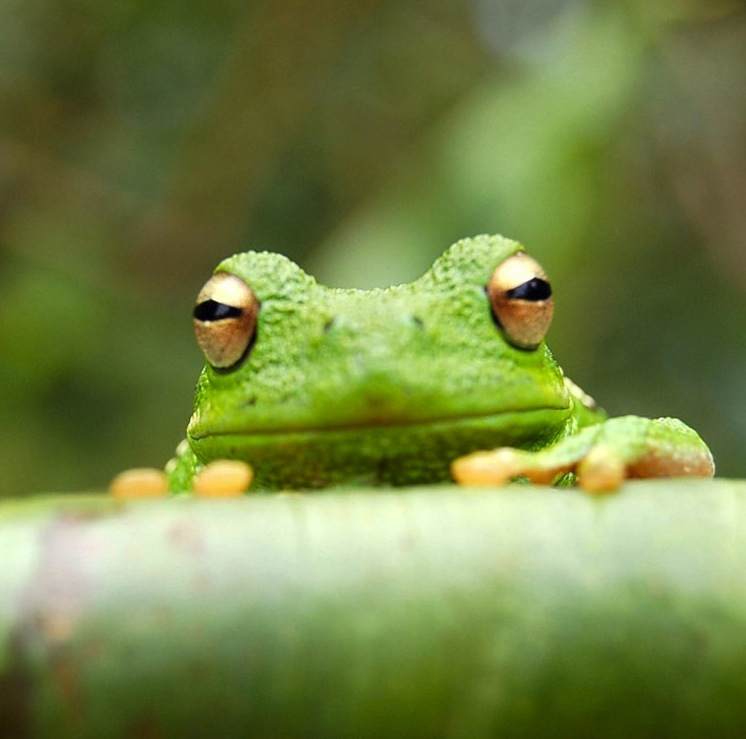
\includegraphics[width=0.3\textwidth]{Chapters/Chapter_4/frog1.jpg}
\caption{\label{fig:frog}This frog was uploaded via the file-tree menu.\cite{textbook}}
\end{figure}
\subsection{How to add table}
Use the table and tabular environments for basic tables --- see Table~\ref{tab:widgets}, for example\cite{article}. For more information, please see this help article on \href{https://www.overleaf.com/learn/latex/tables}{tables}. 

\begin{table}[ht]
\centering
\begin{tabular}{l|r}
Item & Quantity \\\hline
Widgets & 42 \\
Gadgets & 13
\end{tabular}
\caption{\label{tab:widgets}An example table.}
\end{table}

\subsection{How to add Lists}

You can make lists with automatic numbering \dots

\begin{enumerate}
\item Like this,
\item and like this.
\end{enumerate}
\dots or bullet points \dots
\begin{itemize}
\item Like this,
\item and like this.
\end{itemize}

\subsection{How to write Formula}

\LaTeX{} is great at typesetting mathematics. Let $X_1, X_2, \ldots, X_n$ be a sequence of independent and identically distributed random variables with $\text{E}[X_i] = \mu$ and $\text{Var}[X_i] = \sigma^2 < \infty$, and let
\[S_n = \frac{X_1 + X_2 + \cdots + X_n}{n}
      = \frac{1}{n}\sum_{i}^{n} X_i\]
denote their mean. Then as $n$ approaches infinity, the random variables $\sqrt{n}(S_n - \mu)$ converge in distribution to a normal $\mathcal{N}(0, \sigma^2)$.





%%%%%%%%%%%%%%%%% Changes%%%%%%%%%%%%%%%%%%%%%%%%














































